% #############################################################################
% This is Chapter 4
% !TEX root = ../main.tex
% #############################################################################
% Change the Name of the Chapter i the following line
\fancychapter{Aerial-D Dataset Construction}
\cleardoublepage
% The following line allows to ref this chapter
\label{chap:implement}

This section details our comprehensive approach to constructing Aerial-D, a large-scale referring expression segmentation dataset for aerial imagery. Our methodology combines automated rule-based expression generation with a multimodal LLM expression component that is preceded by a cost-efficient distillation step, enabling both scale and linguistic diversity. We begin by establishing our source datasets, then describe our rule-based pipeline for generating referring expressions from existing annotations, followed by our distilled large language model enhancement procedure, and conclude with comprehensive dataset statistics demonstrating the scope and characteristics of the final resource.

% #############################################################################
\section{Source Datasets}

The Aerial-D dataset is constructed from two complementary aerial datasets with different annotation styles: iSAID (instance segmentation) and LoveDA (semantic segmentation), as illustrated in Table~\ref{tab:dataset_sources}.


% Dataset sources table with images
\begin{table}[H]
\centering
\caption{Source Dataset Characteristics}
\label{tab:dataset_sources}
\begin{tabular}{@{}p{4cm}p{8cm}@{}}
\toprule
\multicolumn{2}{c}{\textbf{iSAID Dataset}} \\
\midrule
\raisebox{-0.5\height}{\includegraphics[width=3.5cm, height=3.5cm]{Images/isaid.png}} & 
\hspace{-0.5cm}\parbox[c]{8cm}{\fontsize{10pt}{12pt}\selectfont Contains \textbf{2,806} high resolution images at varying widths of 800 to 13,000 pixels, spatial resolution of \textbf{0.1m to 4.5m}, with \textbf{655,451} instances across \textbf{15} object classes: \textbf{ships}, \textbf{large vehicles}, \textbf{small vehicles}, \textbf{storage tanks}, \textbf{harbors}, \textbf{swimming pools}, \textbf{tennis courts}, \textbf{soccer ball fields}, \textbf{roundabouts}, \textbf{basketball courts}, \textbf{bridges}, \textbf{ground track fields}, \textbf{planes}, \textbf{helicopters}, and \textbf{baseball diamonds}.} \\[0.5cm]
\midrule
\multicolumn{2}{c}{\textbf{LoveDA Dataset}} \\
\midrule
\raisebox{-0.5\height}{\includegraphics[width=3.5cm, height=3.5cm]{Images/loveda_dataset.png}} & 
\hspace{-0.5cm}\parbox[c]{8cm}{\fontsize{10pt}{12pt}\selectfont Contains \textbf{5,987} images at 1024 pixel width, spatial resolution of \textbf{0.3m}, across \textbf{6} land cover classes: \textbf{building}, \textbf{road}, \textbf{water}, \textbf{barren}, \textbf{forest}, and \textbf{agriculture}.} \\[0.5cm]
\bottomrule
\end{tabular}
\end{table}

The lack of accompanying language annotations is the primary limitation of both resources: iSAID delivers dense instance masks but no textual descriptions, while LoveDA supplies per-pixel semantic labels without any natural language explanations. Chapter~\ref{chap:implement} therefore introduces an automated pipeline that augments these geometric annotations with referring expressions at scale, beginning with the rule-based system described next.

% #############################################################################
% #############################################################################
\section{Rule-Based Expression Generation}

Both iSAID and LoveDA deliver rich geometric annotations—instance masks in COCO format on one side, semantic maps on the other—but neither includes the natural language expressions required for referring segmentation. Our first step is therefore to squeeze as much descriptive signal as possible from those annotations alone: we mine every positional, visual, and relational cue we can extract and arrange them into language templates that serve as the initial expression candidates. We refer to this deterministic pipeline as the rule-based generation stage. The pipeline systematically transforms semantic segmentation and instance segmentation datasets into referring expression resources through a sequential process that analyzes spatial, visual, and relational properties of objects and groups within aerial imagery. The development of these rules emerged through extensive experimentation and empirical analysis, where we iteratively observed cases of ambiguity in generated expressions and refined the rule parameters until the most challenging edge cases were resolved. This comprehensive approach begins with patch extraction from source datasets and culminates in linguistically diverse and contextually accurate referring expressions. At a high level, it advances through the following stages:
\begin{enumerate}[label=\textbf{\arabic*.}, leftmargin=*]
    \item \textbf{Patch Preparation}: extracts 480$\times$480 patches from iSAID using a sliding window with overlap and resizes LoveDA tiles while converting select semantic classes into instance masks.
    \item \textbf{Grid Position Assignment}: partitions each patch into a three-by-three grid and handles borderline cases with multiple valid positional labels.
    \item \textbf{Color and Visual Attributes}: classifies object colors in HSV space with dominance thresholds and suppresses noisy cues for categories with unreliable chromatic signals.
    \item \textbf{Extreme Position Detection}: identifies topmost, bottommost, leftmost, and rightmost instances within each category using separation margins that avoid ambiguous ties.
    \item \textbf{Spatial Relationship Extraction}: computes angle-based relationships between nearby objects using adaptive distance thresholds to capture meaningful relative positioning.
    \item \textbf{Group Formation}: clusters nearby instances with DBSCAN, assigns group-level attributes, and supports relationships across instance and group combinations.
    \item \textbf{Expression Synthesis and Filtering}: combines all attributes through templated generation and removes duplicate expressions to ensure each phrase uniquely refers to a single target.
\end{enumerate}

\begin{figure}[H]
\centering
\begin{minipage}{0.5\textwidth}
\centering
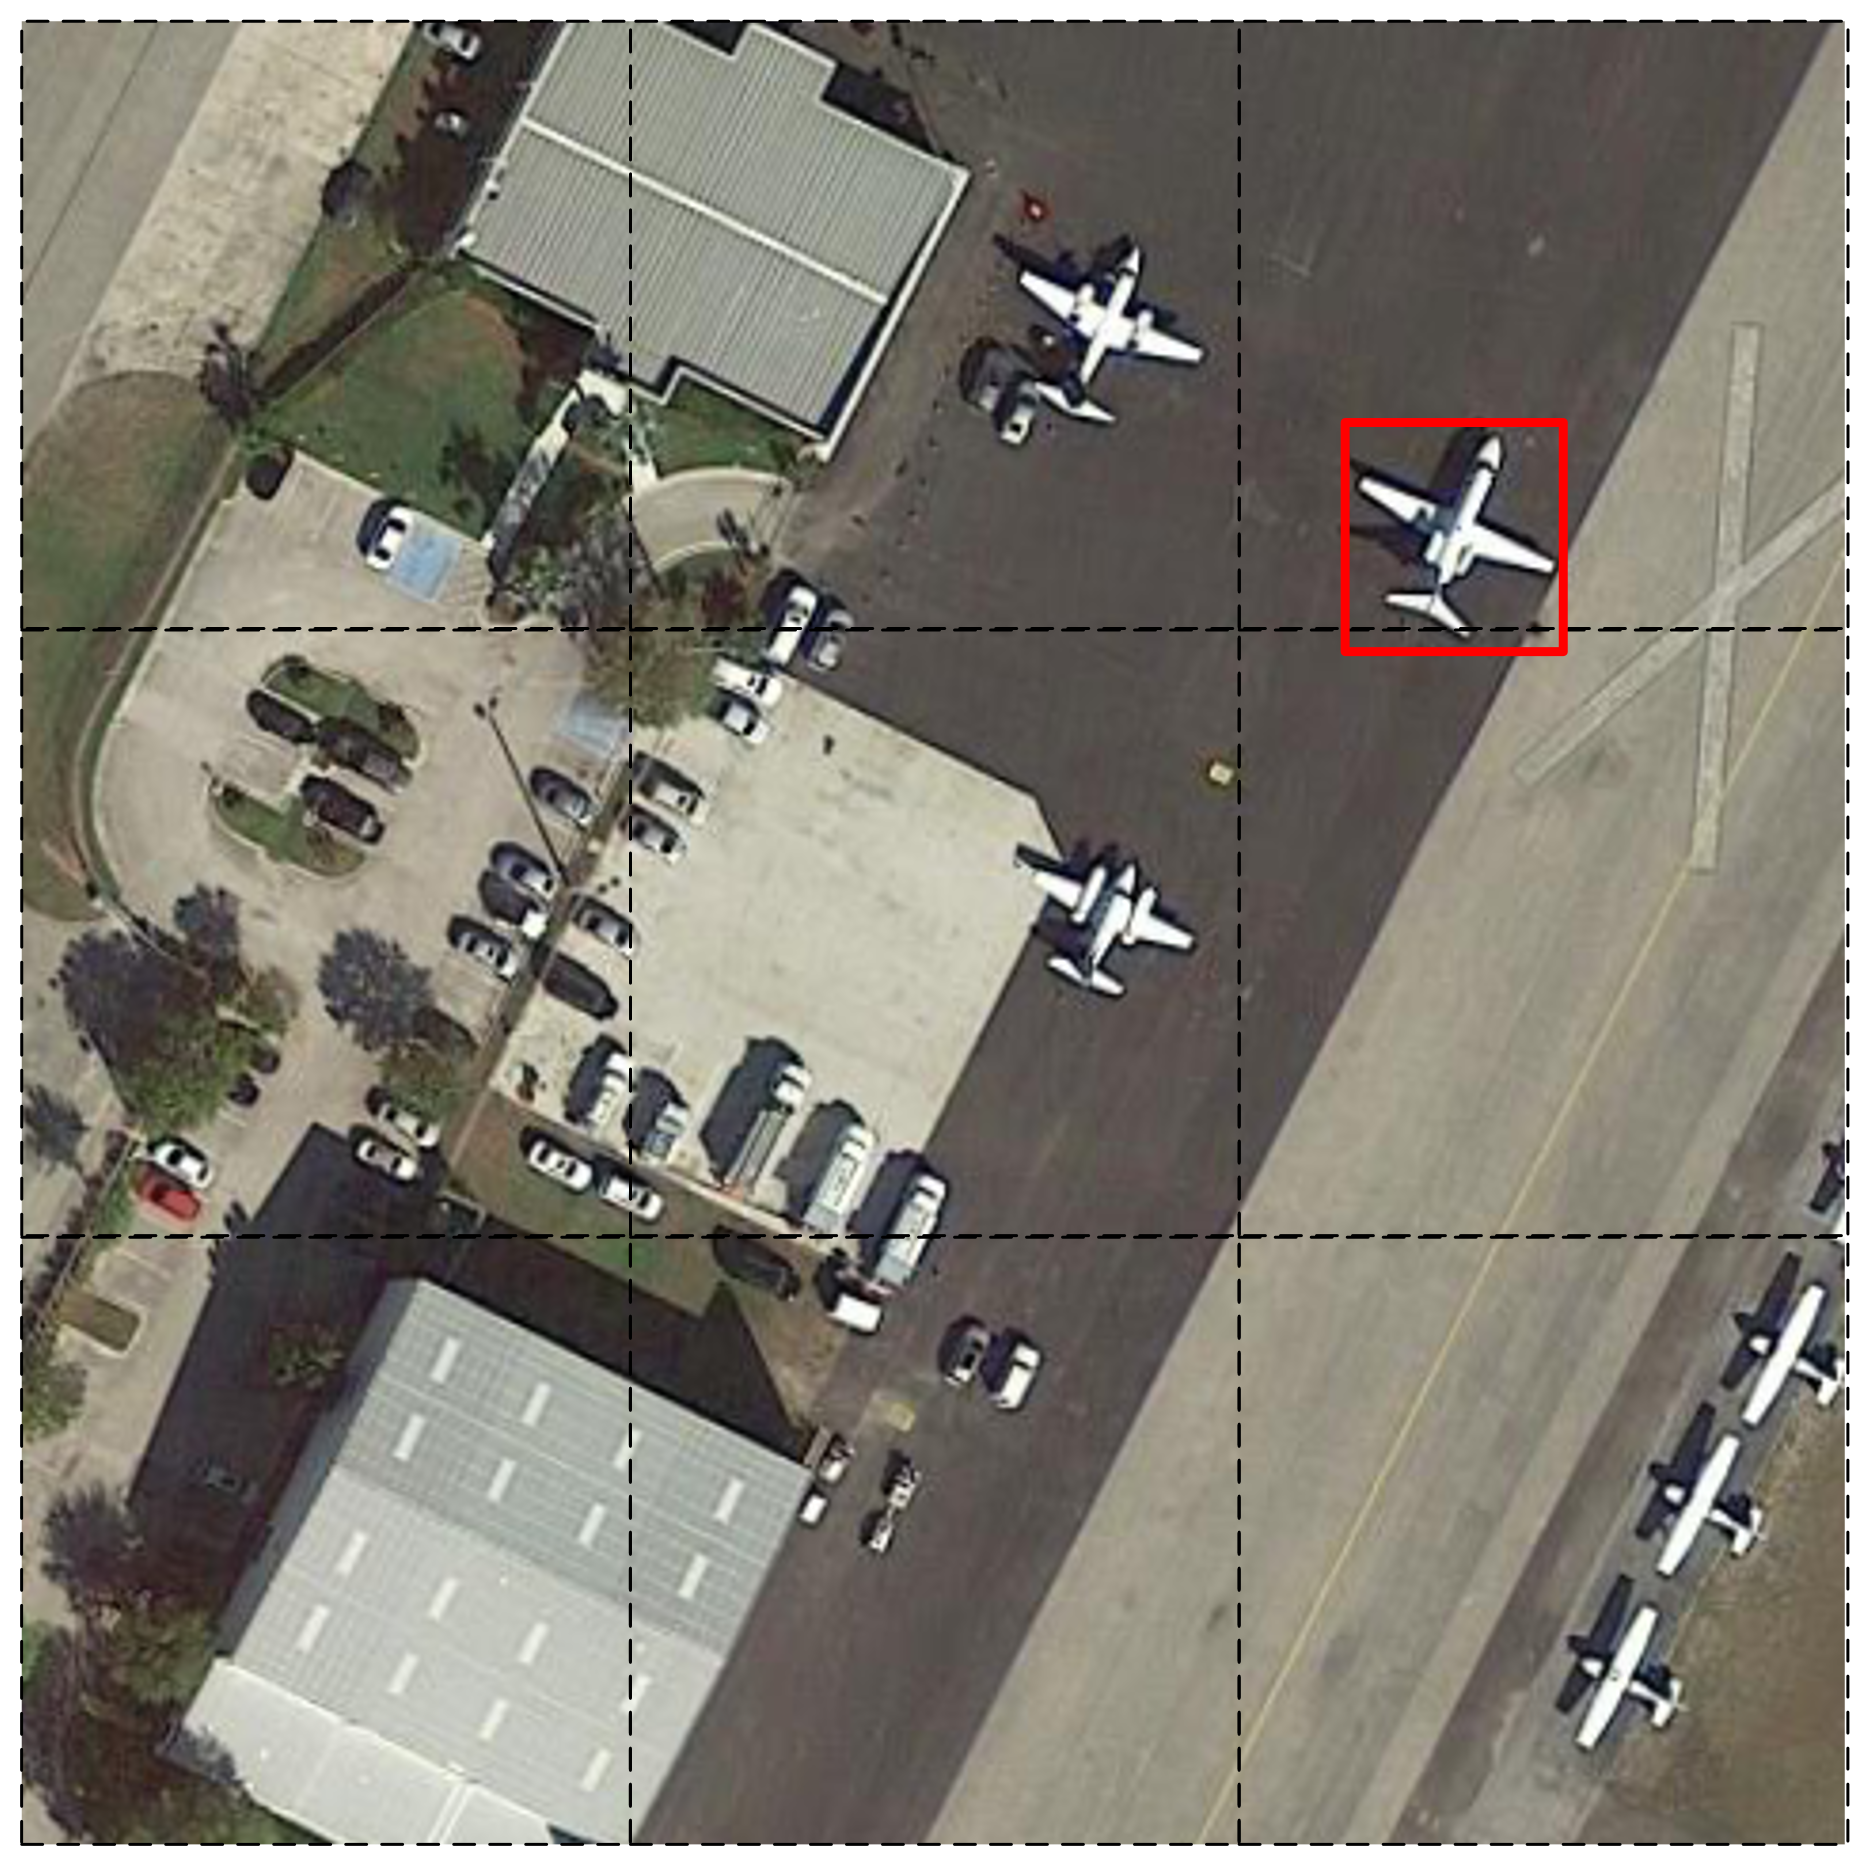
\includegraphics[width=0.7\textwidth]{Images/rule_based_generation.png}
\end{minipage}%
\begin{minipage}{0.5\textwidth}
\centering
\hspace{-1cm}
\raisebox{-0.3\height}{%
\resizebox{\textwidth}{!}{%
\footnotesize
\begin{tabular}{@{}ll@{}}
\toprule
\textbf{Rule Type} & \textbf{Example Instance} \\
\midrule
Category & "plane" \\
Grid Position & "in the top right" \\
Extreme Position & None \\
Color Classification & "light" \\
Directional Relations & "to the bottom right of a plane" \\
& "to the top right of a plane" \\
\midrule
\multicolumn{2}{l}{\textbf{Final Expressions}} \\
\multicolumn{2}{l}{"the plane in the top right"} \\
\multicolumn{2}{l}{"the light plane in the top right"} \\
\multicolumn{2}{l}{"the plane in the top right to the bottom right of a plane"} \\
\multicolumn{2}{l}{"the light plane in the top right to the bottom right of a plane"} \\
\multicolumn{2}{l}{"the plane in the top right to the top right of a plane"} \\
\multicolumn{2}{l}{"the light plane in the top right to the top right of a plane"} \\
\bottomrule
\end{tabular}%
}%
}
\end{minipage}
\caption{Example of rule generation for a single instance. The highlighted plane in the top right section demonstrates how the system assigns spatial, visual, and relational rules that will later be combined into referring expressions.}
\label{fig:rule_example}
\end{figure}

\subsubsection{iSAID Patch Extraction}
The process initiates with iSAID patch extraction, where instance annotations are loaded from COCO-format JSON files containing 655,451 instances across 15 object categories. The system extracts 480$\times$480 patches using a sliding window approach with 20\% overlap, processing both training and validation splits through multiprocessing for computational efficiency. The sliding window approach creates the risk that objects may be partially cut off at patch boundaries, where a cutoff object is defined as an instance whose segmentation polygon extends beyond the extracted patch area. Critical to maintaining annotation quality, the extraction process handles cutoff objects by calculating intersection ratios, marking instances where less than 50\% remains within patch boundaries and fewer than 500 pixels are visible as potentially unreliable. Polygon segmentations are converted to run-length encoding (RLE) format for storage efficiency, while we extract essential metadata from JSON annotations including bounding boxes, areas, and segmentation data. The system filters out patches with excessive black pixels exceeding a 50\% threshold, ensuring visual content quality throughout the dataset.

\subsubsection{LoveDA Patch Processing}
LoveDA patch processing follows a distinct approach tailored to semantic segmentation data from 1024$\times$1024 images across urban and rural domains. The system resizes the entire image to 480$\times$480 dimensions to maintain consistency with iSAID patches. For ``building'' and ``water'' categories, the system converts semantic segmentation masks into individual instance segmentation masks through connected components analysis. This selective conversion makes sense because LoveDA's land cover classification design means that buildings and water bodies naturally occur as discrete, spatially bounded entities with clear geometric boundaries, making them suitable for instance segmentation. In contrast, classes such as agriculture, forest, and barren land represent diffuse land cover types that extend across large continuous regions without natural instance boundaries, making individual instance extraction neither meaningful nor reliable for these categories.

\subsubsection{Connected Components Analysis}
The connected components analysis identifies spatially connected regions within each semantic class by examining pixel connectivity patterns. The algorithm traverses the binary mask where pixels are considered connected if they are adjacent horizontally, vertically, or diagonally, meaning each pixel can connect to any of its eight neighboring pixels in the surrounding 3$\times$3 grid, effectively grouping contiguous pixels belonging to the same semantic class into distinct labeled regions. Connected components below minimum area thresholds of 50 pixels for buildings and 100 pixels for water are filtered out to eliminate spurious detections. This dual-layer processing creates both individual building and water instances for referring expression generation, while simultaneously preserving the complete semantic segmentation masks containing all pixels of each class. Agricultural areas, forests, and barren land are exclusively treated as unified semantic classes, with single masks encompassing all pixels of each category and pre-written expressions such as ``all buildings in the image'' generated for these class-level groups, while multiprocessing handles both urban and rural domains efficiently.

\subsubsection{Rule Addition and Analysis}
Having established 480$\times$480 patches with annotated object instances and masks from both iSAID and LoveDA processing, the pipeline proceeds to the core rule addition and analysis phase, which transforms these basic annotations into rich spatial and visual descriptions through systematic feature extraction. Each 480$\times$480 patch undergoes partitioning into a three-by-three grid establishing nine distinct spatial regions, as illustrated in Figure \ref{fig:rule_example}. The grid divides the image into equal thirds both horizontally and vertically, creating regions such as ``top left'', ``center'', and ``bottom right''. However, objects positioned near grid boundaries present a challenge, as instances separated by just a few pixels between adjacent regions could create ambiguity in referring expressions and confuse models about which specific object is being referenced. To address this boundary ambiguity, the system implements borderline detection using a boundary threshold of 10\% of the image dimensions. When an object's centroid falls within this boundary zone (48 pixels from any grid line in a 480$\times$480 image), the system generates multiple valid position labels for that instance. For example, an object near the boundary between ``top center'' and ``center center'' regions receives both position labels as valid alternatives. This dual-labeling strategy ensures robust expression generation, as conflicting expressions referencing the same borderline object will be filtered out in subsequent deduplication steps, while maintaining coverage for legitimate spatial references.

\subsubsection{Color Classification}
To provide comprehensive visual features for referring expressions, the system performs color classification for each individual object instance. The classification process operates on HSV color space pixels extracted from segmentation masks, first distinguishing between achromatic and chromatic colors through saturation analysis. Objects are classified as achromatic when their saturation levels fall below 25\%, further subdivided into light and dark categories using a brightness threshold of 54\%. For chromatic instances, the system identifies specific hue ranges across eight distinct colors: red, orange, yellow, green, cyan, blue, purple, and magenta, with each hue occupying predetermined angular ranges within the HSV color wheel. The system requires 70\% dominance thresholds for both achromatic and chromatic classifications to ensure reliable color assignment. However, for buildings and water instances, chromatic color references are filtered out during expression generation, as these objects typically exhibit random, multi-hue color patterns that do not provide meaningful discriminative information for referring expressions. The system does not assign colors to every instance, particularly in cases where multiple hues are present within a single object or when the color distribution is ambiguous, as assigning incorrect color labels could create misleading referring expressions.

\subsubsection{Extreme Position Detection}
In order to provide additional spatial context beyond grid positioning, the system introduces extreme position detection to identify instances that occupy boundary locations within their respective object categories. This analysis proves particularly valuable for scenes containing multiple objects of the same type, where conventional grid-based positioning may be insufficient for unique identification. The system determines topmost, bottommost, leftmost, and rightmost instances within each category by first sorting objects by their centroid coordinates, then applying a separation threshold to ensure meaningful distinctions. Specifically, the system uses a margin ratio of 5\% of the image dimensions (24 pixels in a 480$\times$480 image) to verify that the most extreme object is sufficiently separated from the second-most extreme object before assigning the extreme position label. For example, for topmost detection, the system compares the y-coordinates of the two highest objects and only assigns the ``topmost'' label if their vertical separation exceeds the margin threshold, enabling reliable expressions such as ``the leftmost ship'' or ``the topmost building'' when multiple instances of the same class are present.

\subsubsection{Spatial Relationship Calculation}
To enable complex referring expressions that describe objects in terms of their proximity to other instances, the system implements spatial relationship calculation. This addresses cases where objects need to be localized relative to nearby instances within the scene, particularly when absolute grid positions alone cannot provide sufficient discriminative information. The system employs an angle-based directional system calculating angular relationships between object centroids to determine relative positioning using eight distinct directions: to the left of, to the bottom left of, below, to the bottom right of, to the right of, to the top right of, above, and to the top left of. However, establishing relationships between all possible object pairs would create spurious connections between distant objects that provide no meaningful spatial context for referring expressions, potentially leading to confusing references like "the ship to the left of a building" when the building is at the opposite edge of the image. To address this problem, the system limits relationships to nearby instances using dynamic distance thresholds rather than fixed distances. A fixed threshold would incorrectly discard meaningful relationships involving large objects, such as when a vehicle appears to the left of a large roundabout whose centroid lies at its geometric center - the fixed distance from the vehicle to the roundabout's centroid might exceed the threshold despite their obvious spatial relationship. The dynamic threshold starts with a base maximum distance of 150 pixels, then adds half the average size of both source and target objects to account for object scale. For example, when relating two large buildings with average dimensions of 60 pixels, the maximum relationship distance becomes 210 pixels (150 + 30 + 30), ensuring that larger objects can establish relationships across greater distances than smaller objects while preventing meaningless long-distance connections. When objects fall near angular boundaries between directional zones, the system handles these borderline cases by recording multiple directional possibilities, similar to the absolute grid positioning borderline detection, ensuring comprehensive coverage of spatial interpretations and preventing arbitrary assignment decisions.

\subsubsection{Group Formation}
To handle scenarios where multiple instances of the same object category appear within patches, the system introduces group formation to enable collective referring expressions and reduce annotation redundancy. This addresses the challenge of creating natural language expressions when numerous similar objects are present, where individual instance references would become unwieldy or ambiguous. The system utilizes DBSCAN clustering~\cite{dbscan} with carefully tuned parameters: epsilon distance of 40 pixels, minimum cluster size of 2 objects, and maximum cluster size of 8 objects, operating separately within each object category to maintain semantic coherence. The clustering algorithm employs minimum edge distance between bounding boxes rather than centroid distance to determine which instances should be grouped together. This bounding box distance approach calculates the shortest distance between the edges of two object rectangles, returning zero when boxes overlap and the actual gap distance when they are separated. This method provides a more accurate representation of spatial proximity for clustering purposes, as two large objects with distant centroids but touching edges should logically be grouped together, while two small objects with close centroids but separated by a gap should remain distinct. Class-level groups are automatically generated for categories containing multiple instances, creating expressions such as ``all ships in the image'' when numerous instances of the same type are present. Additionally, the system creates special pair groups that combine small and large vehicles when both vehicle types coexist within patches, enabling more natural referring expressions that reference vehicle collections rather than individual instances. Groups receive their own position rules based on calculated group centroids and can establish relationships with other groups and individual instances. The system supports three distinct types of relationships: instance-to-instance relationships between individual objects, group-to-group relationships between clustered entities, and instance-to-group relationships that allow individual objects to be described relative to nearby groups. This enables natural language expressions that can reference objects in relation to both individual instances and collective groups, providing rich contextual information for complex aerial scenes.

\subsubsection{Expression Synthesis}
Having extracted all spatial, visual, and relational attributes for individual instances and established groups of instances through clustering, the system now synthesizes these components into actual referring expressions. As demonstrated in the table within Figure \ref{fig:rule_example}, the expression generation process systematically combines all available rules and attributes to create comprehensive linguistic descriptions. The system takes each extracted rule type and generates all valid combinations, creating expressions that range from simple category-only descriptions like ``the ship'' to complex multi-attribute formulations such as ``the dark ship in the top right that is above a harbor''. The combinatorial approach ensures thorough coverage of all possible referring expressions by systematically enumerating combinations of category labels, grid positions, spatial relationships, extreme positions, size characteristics, and color properties across seventeen distinct expression templates. For group expressions, the system handles multi-instance clusters with appropriate size quantifiers and plural forms, enabling natural references to collections of objects. During this process, the system also converts class names from technical formats to natural language equivalents, transforming ``Large\_Vehicle'' to ``large vehicle'' and applying appropriate pluralization logic based on group sizes and context. Additionally, the system generates dummy expressions for instances that are borderline or marked as cut off at patch boundaries, maintaining these potentially unreliable expressions specifically to avoid ambiguity during the subsequent filtering process described next.

% Expression uniqueness filter example
\begin{figure}[H]
\centering
\begin{minipage}{0.5\textwidth}
\centering
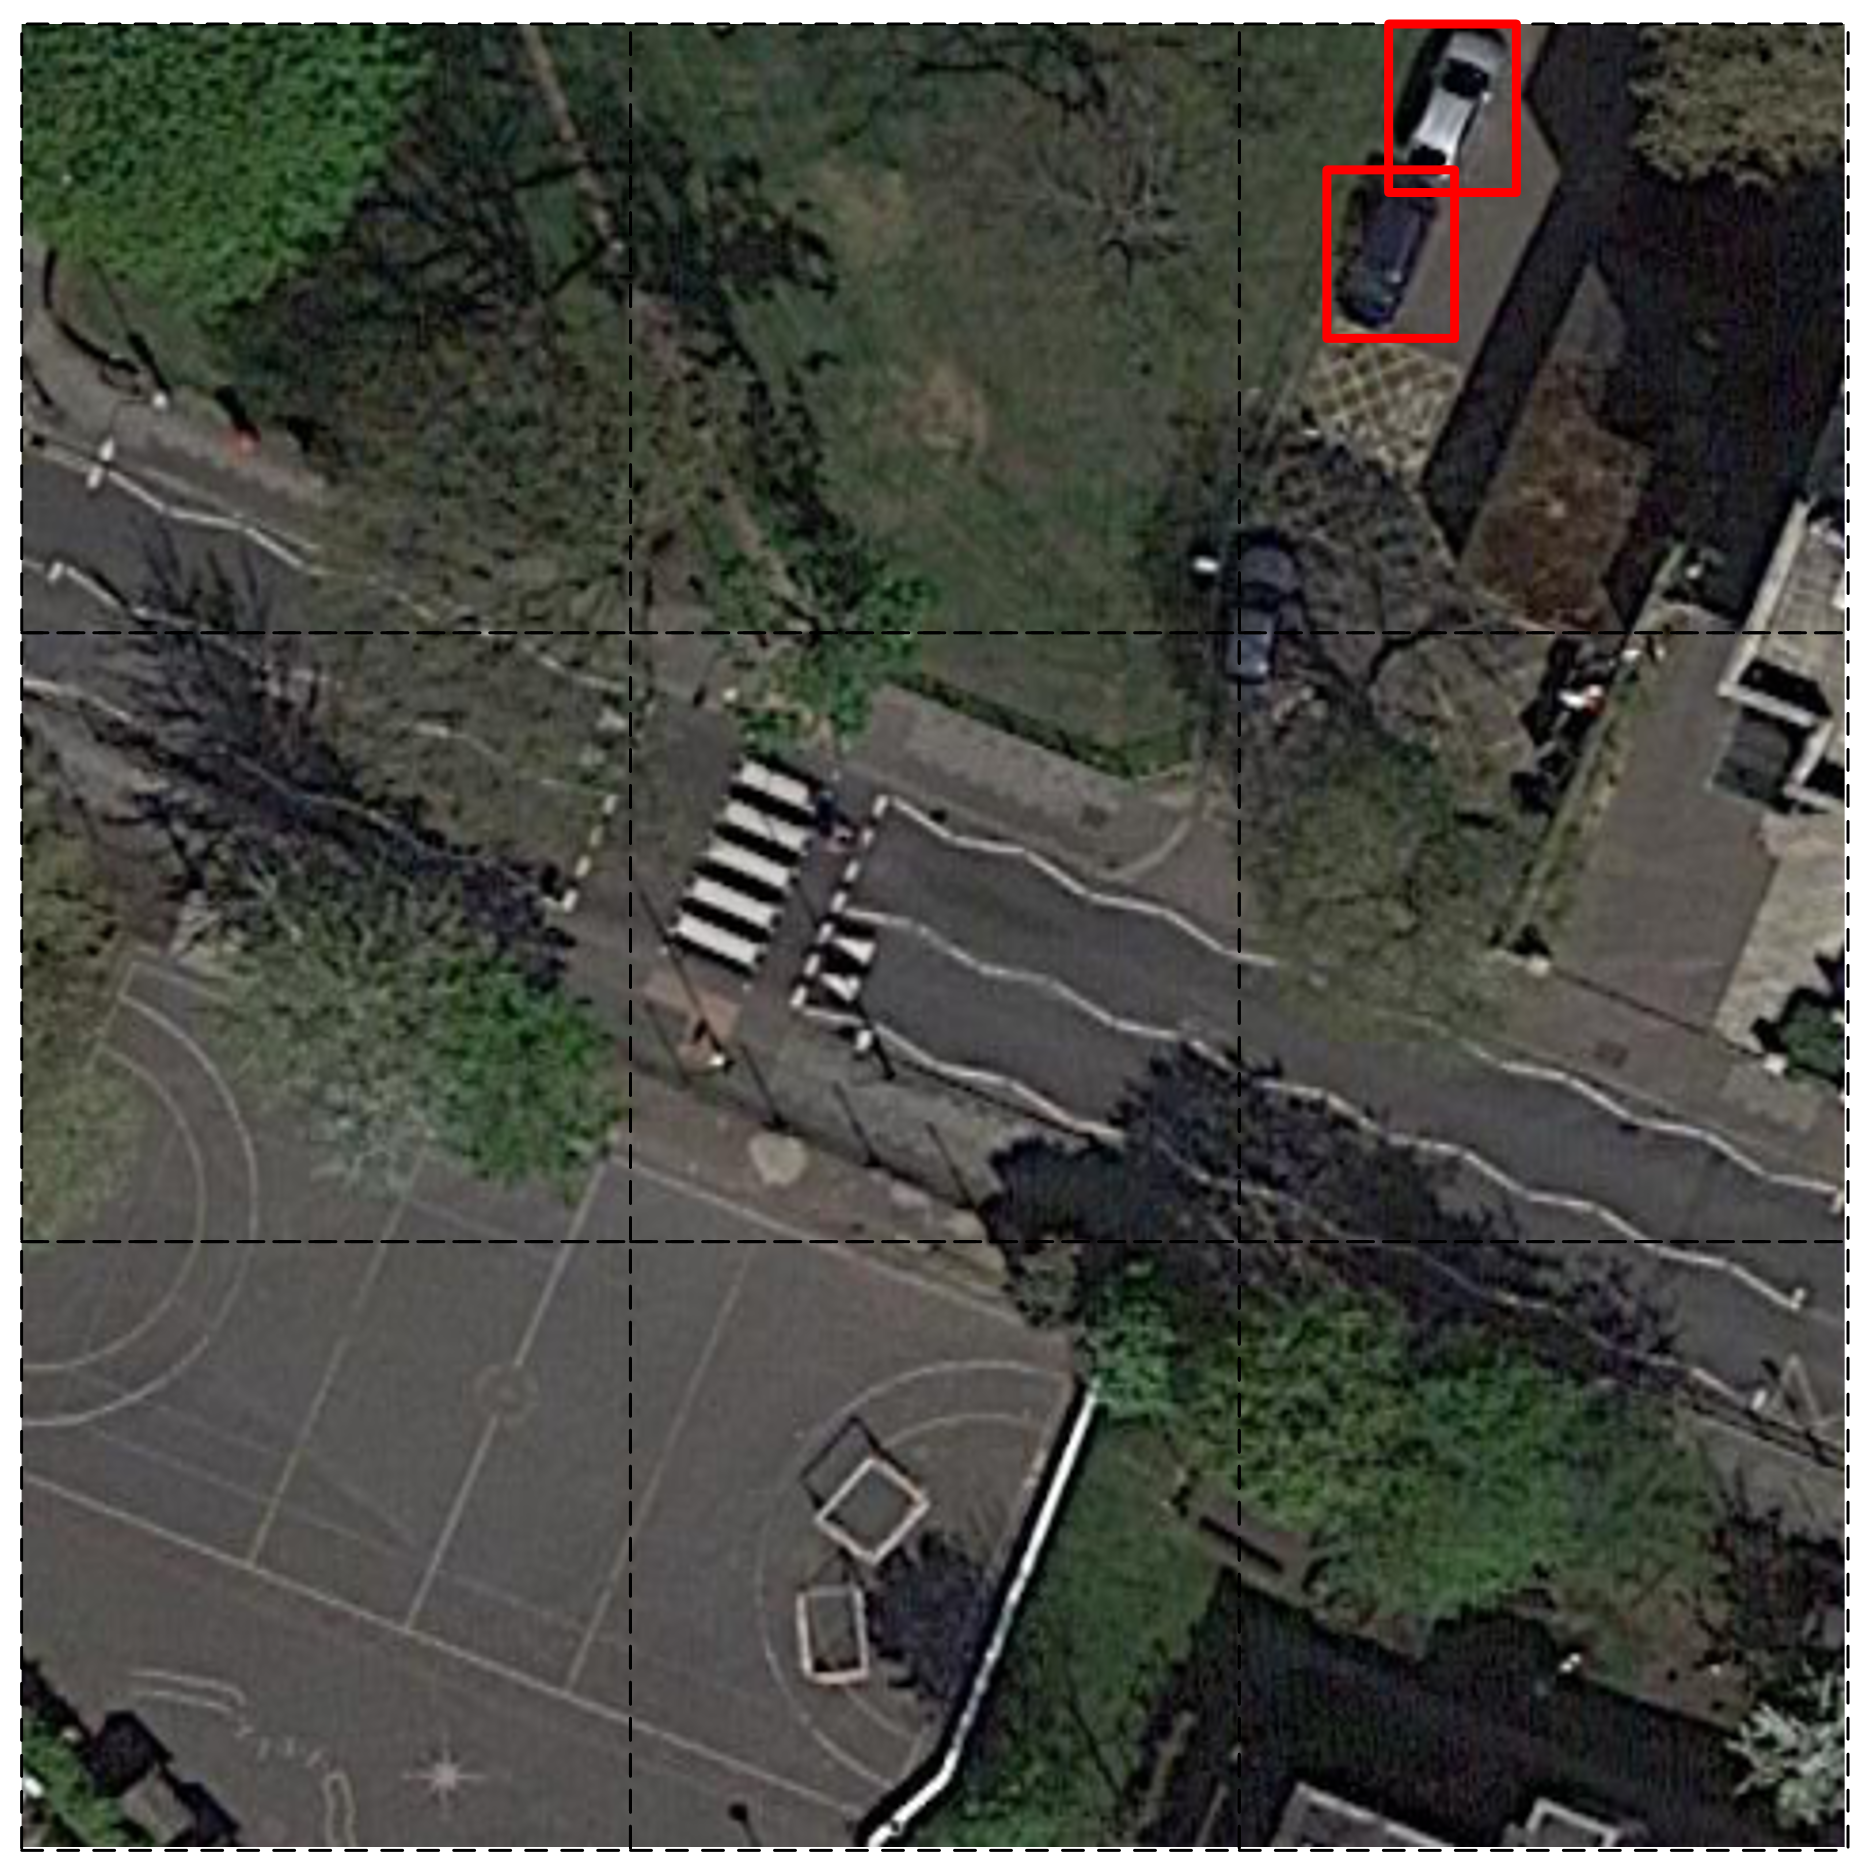
\includegraphics[width=0.7\textwidth]{Images/filter_unique.png}
\end{minipage}%
\begin{minipage}{0.5\textwidth}
\centering
\hspace{-1cm}
\raisebox{-0.3\height}{%
\resizebox{\textwidth}{!}{%
\footnotesize
\begin{tabular}{@{}ll@{}}
\toprule
\textbf{Expression} & \textbf{Status} \\
\midrule
\multicolumn{2}{l}{\textbf{Object 1 (Light Vehicle)}} \\
\midrule
"the small vehicle in the top right" & \textcolor{red}{Filtered} \\
"the topmost small vehicle" & \textcolor{green!70!black}{Kept} \\
"the light small vehicle in the top right" & \textcolor{green!70!black}{Kept} \\
"the light topmost small vehicle" & \textcolor{green!70!black}{Kept} \\
"the small vehicle in the top right above a small vehicle" & \textcolor{green!70!black}{Kept} \\
\midrule
\multicolumn{2}{l}{\textbf{Object 2 (Dark Vehicle)}} \\
\midrule
"the small vehicle in the top right" & \textcolor{red}{Filtered} \\
"the dark small vehicle in the top right" & \textcolor{green!70!black}{Kept} \\
"the small vehicle in the top right below a small vehicle" & \textcolor{green!70!black}{Kept} \\
\bottomrule
\end{tabular}%
}%
}
\end{minipage}
\caption{Example of expression uniqueness filtering. When two objects share similar attributes, conflicting expressions like "the small vehicle in the top right" are filtered out, while unique expressions that distinguish between objects are retained.}
\label{fig:filter_unique_example}
\end{figure}

\subsubsection{Uniqueness Filtering}
The fundamental problem that emerges from comprehensive expression generation is the creation of conflicting expressions, as illustrated in Figure \ref{fig:filter_unique_example}. When two objects possess identical attributes and rules, they inevitably generate some expressions that are exactly the same, creating ambiguous references where a single phrase could refer to multiple different objects. For example, if two vehicles share the same grid position, expressions like ``the small vehicle in the top right'' become ambiguous and compromise the referring expression task. To resolve this ambiguity, the system implements uniqueness filtering, which systematically identifies and removes all expressions that appear multiple times across the dataset. The strict deduplication policy eliminates all occurrences of non-unique phrases, ensuring that every remaining expression uniquely identifies a single object or group. This is precisely where dummy expressions prove essential: when borderline cases generate multiple valid position labels, relationship directions, or other ambiguous attributes, these alternative expressions naturally cancel each other out during filtering, leaving only the unambiguous expressions that provide clear, unique references. Objects and groups that lose all their expressions during this filtering process are eliminated entirely from the dataset, maintaining only high-confidence annotations with reliable referring expressions.


% #############################################################################
\section{LLM Expression Generation}
\label{subsec:llm_expression_generation}

While rule-based expression generation provides a solid foundation for referring expression data, these expressions suffer from significant limitations in language variation and visual detail coverage. The rule-based approach produces linguistically constrained expressions with limited wording variations and lacks the ability to reference contextual elements beyond predefined source dataset categories.

To address these limitations, we employ a multimodal Large Language Model (LLM) to enhance our dataset by providing both images and expressions as input, enabling the model to rewrite and improve the original referring expressions. We prompt the LLM with two complementary tasks, as shown in Figure \ref{fig:llm_enhancement_example} and detailed in Appendix~A. The first task focuses on linguistic variation, creating natural language alternatives for each rule-based expression without heavy reliance on visual cues. The second task uses visual information, where the model examines surrounding features in the image around the target object.

To ensure the LLM accurately identifies and describes the target region, we employ a sophisticated visual prompting strategy that adapts to different target types. For discrete objects and groups, we overlay the target region with red bounding boxes that visually highlight the area of interest, guiding the model's attention during generation. Each prompt includes both the full 480×480 image patch and a focused close-up crop centered on the target, which proves essential for small or densely packed objects that might occupy only a few pixels in the original view. For land-cover categories such as vegetation, agriculture, or water that extend across irregular regions without clear bounding boxes, we employ a dual-image prompting technique: the first image shows the original scene with a semi-transparent color overlay masking the target region, while the second image presents the clean unmasked view. This paired presentation helps the LLM anchor its understanding to the relevant semantic region while maintaining awareness of the surrounding context. The combination of bounding box overlays for instance targets, close-up crops for fine details, and dual-image mask prompts for semantic regions ensures the enhancement remains spatially grounded and accurate across all target types in the dataset.

This dual-task prompting transforms basic expressions like "the group of 4 large vehicles in the top center" into linguistically diverse alternatives such as "the cluster of four big vehicles near the upper middle" and visually detailed descriptions like "the four large vehicles lined up side by side just below the pale paved strip at the very top middle", as shown in Figure~\ref{fig:llm_enhancement_example}. The model identifies and references contextual elements not captured in the original datasets, such as the "pale paved strip" and the "grassy area".

% LLM enhancement example figure
\begin{figure}[t]
\centering
\begin{minipage}{0.5\textwidth}
\centering
\includegraphics[width=0.7\textwidth]{Images/example_group.png}
\end{minipage}%
\begin{minipage}{0.5\textwidth}
\centering
\hspace{-1cm}
\raisebox{-0.3\height}{%
\footnotesize
\begin{tabular}{@{}p{2cm}p{5cm}@{}}
\toprule
\textbf{Expression Type} & \textbf{Example} \\
\midrule
Original & the group of 4 large vehicles in the top center \\
\midrule
Enhanced & the cluster of four big vehicles near the upper middle \\
\midrule
Unique & the four large vehicles lined up side by side just below the pale paved strip at the very top middle \\
\midrule
Unique & the set of four big vehicles parked in a single row in the upper center beside the grassy area to the right \\
\bottomrule
\end{tabular}%
}
\end{minipage}
\caption{Example of LLM enhancement process showing original aerial image with group of four large vehicles (left) and corresponding expression enhancements (right).}
\label{fig:llm_enhancement_example}
\end{figure}

However, the full dataset contains approximately 300,000 captured targets including both objects and groups. To generate expressions, we process each target individually, meaning we would need 300,000 separate LLM requests. Using production-grade LLMs at this scale—for example, OpenAI's o3 model\cite{o3} with strong visual capabilities—would cost thousands of dollars; Table \ref{tab:cost_comparison} reports the exact breakdown, making direct application prohibitively expensive for research-scale dataset construction.

To address this scalability challenge, we employ a knowledge distillation approach, as illustrated in Figure \ref{fig:llm_distillation}. We utilize OpenAI's o3 model\cite{o3} and compare it against a much more lightweight open‑weights model, Gemma3\cite{gemma3}. We obtain 500 high‑quality outputs from o3 on a representative random subset of targets from the initial dataset. These outputs serve as training data for supervised fine‑tuning using the parameter‑efficient QLoRA method\cite{qlora} on Gemma3‑12B.

During fine-tuning we apply LoRA adapters across both the text decoder and the SigLIP-derived vision stack embedded in Gemma3, which improves instruction adherence, suppresses hallucinations, and stabilises the two-task output schema. The custom-tailored Gemma3 variant can then process all 300,000 targets on a single GPU while honouring the dual-task prompt structure—behaviour the base Gemma3 model fails to follow reliably without distillation. Notably, the distilled model's output quality approaches o3's once fine‑tuned; qualitative comparisons in Figure \ref{fig:distillation_comparison} show closely matched enhancements with markedly reduced hallucinations relative to the base Gemma3 model.

\begin{figure}[t]
\centering
\includegraphics[width=\columnwidth]{Images/distillation.png}
\caption{Knowledge distillation pipeline for scalable LLM enhancement. A small sample of 500 expressions is processed through OpenAI's o3 model\cite{o3} to generate high-quality training targets, which are then used to fine-tune Gemma3‑12B\cite{gemma3} via QLoRA\cite{qlora}. The fine‑tuned model enables cost‑effective local inference to enhance the full dataset using vLLM\cite{vllm} on a single GPU.}
\label{fig:llm_distillation}
\end{figure}

% #############################################################################
\section{Historic Image Filters}
\label{subsec:historic_filters}

In order to keep the dataset useful for models that must operate on archival imagery, we simulate the visual signatures that appear in mid-century aerial collections. Historic film stocks and scanning workflows frequently desaturate colours, compress tonal range, and inject grain, which diminishes the sharp visual cues that modern networks rely upon. To counter this gap between training data and deployment conditions, we apply three parametric transformations that recreate monochrome capture, film fading with grain, and sepia scanning artifacts for every patch.

Let $I_{\text{orig}}(x) \in [0,255]^3$ denote the RGB vector at pixel $x$, and let $\operatorname{clip}(\cdot)$ clamp intensities to the $[0,255]$ range. We first approximate the luminance response of black-and-white film, producing the grayscale target in Equation~\ref{eq:historic_gray}:
\begin{equation}
I_{\text{gray}}(x) = 0.299\,R(x) + 0.587\,G(x) + 0.114\,B(x).
\label{eq:historic_gray}
\end{equation}
Film reproduction is then mimicked by a sequence of tone adjustments. We apply a mild gamma curve in Equation~\ref{eq:historic_gamma}, recenter contrast around the patch mean $\mu$ in Equation~\ref{eq:historic_contrast}, and finally add zero-mean Gaussian noise in Equation~\ref{eq:historic_grain} to replicate silver-halide grain:
\begin{equation}
I_{\gamma}(x) = 255\left( \frac{I_{\text{gray}}(x)}{255} \right)^{\gamma},
\label{eq:historic_gamma}
\end{equation}
\begin{equation}
I_{c}(x) = \big(I_{\gamma}(x) - \mu\big)\,c + \mu,
\label{eq:historic_contrast}
\end{equation}
\begin{equation}
I_{\text{grain}}(x) = \operatorname{clip}\big(I_{c}(x) + \eta(x)\big), \quad \eta(x) \sim \mathcal{N}(0, \sigma^2).
\label{eq:historic_grain}
\end{equation}
The augmentation uses $\gamma = 1.1$, $c = 0.85$, and $\sigma = 0.1\times 255$ so that contrast is gently reduced while a perceptible grain pattern emerges without obscuring object boundaries.

Sepia scanning artifacts are reproduced by applying the linear colour transform in Equation~\ref{eq:historic_sepia}, followed by uniform sensor noise in Equation~\ref{eq:historic_sepia_noise} to emulate digitisation errors:
\begin{equation}
\begin{bmatrix}
S_R(x) \\
S_G(x) \\
S_B(x)
\end{bmatrix}
= \operatorname{clip}\left(
\begin{bmatrix}
0.272 & 0.534 & 0.131 \\
0.349 & 0.686 & 0.168 \\
0.393 & 0.769 & 0.189
\end{bmatrix}
\begin{bmatrix}
R(x) \\
G(x) \\
B(x)
\end{bmatrix}
\right),
\label{eq:historic_sepia}
\end{equation}
where $\mathbf{S}(x) = [S_R(x), S_G(x), S_B(x)]^\top$.
\begin{equation}
I_{\text{sepia}}(x) = \operatorname{clip}\big(\mathbf{S}(x) + \xi(x)\big), \quad \xi(x) \sim \mathcal{U}(0, 50).
\label{eq:historic_sepia_noise}
\end{equation}
Together these transformations compress colour information, soften tonal contrast, and inject characteristic noise while preserving the spatial layout that segmentation relies upon. Figure~\ref{fig:historic_filters} illustrates the qualitative impact on representative patches.

\begin{figure}[H]
\centering
\includegraphics[width=0.9\textwidth]{Images/filters.png}
\caption{Comparison of original aerial image patch with three historic filter transformations: grayscale conversion, sepia toning, and Gaussian noise addition. These filters simulate common degradation patterns in historical aerial photography.}
\label{fig:historic_filters}
\end{figure}


% #############################################################################
\section{Final Dataset Statistics}

The completed Aerial-D dataset represents a comprehensive resource for aerial referring expression segmentation, containing over 1.5 million expressions across diverse object categories and linguistic patterns. As demonstrated in Figure \ref{fig:dataset_examples}, the final dataset showcases the broad range of instances, groups, and semantic categories enhanced through our multi-stage pipeline, with LLM-generated expressions providing rich visual details and contextual references that extend far beyond the original rule-based templates.

% Dataset examples figure
\begin{figure}[H]
\centering
\includegraphics[width=\textwidth]{Images/dataset.png}
\caption{Representative examples from Aerial-D dataset showing diverse referring expressions with corresponding aerial images and ground truth masks.}
\label{fig:dataset_examples}
\end{figure}

Table \ref{tab:dataset_stats} presents the overall dataset composition, revealing 37,288 total patches containing 259,709 annotated samples with expressions. The dataset maintains a balanced distribution between individual objects (128,715 instances with 889,354 expressions) and groups (130,994 groups with 633,169 expressions), with an average of approximately 7 expressions per individual object and 5 expressions per group. The substantial scale demonstrates the comprehensive coverage achieved through our systematic generation pipeline.

% Dataset statistics table
\begin{table}[H]
\centering
\caption{Dataset Statistics Summary}
\label{tab:dataset_stats}
\begin{tabular}{@{}lrrr@{}}
\toprule
\textbf{Metric} & \textbf{Train} & \textbf{Val} & \textbf{Total} \\
\midrule
Total Patches & 27,480 & 9,808 & 37,288 \\
Individual Objects with Expressions & 94,179 & 34,536 & 128,715 \\
Individual Expressions & 646,686 & 242,668 & 889,354 \\
Groups with Expressions & 96,832 & 34,162 & 130,994 \\
Group Expressions & 471,108 & 162,061 & 633,169 \\
Total Samples & 191,011 & 68,698 & 259,709 \\
Avg. Expressions per Individual Object & 6.87 & 7.03 & 6.91 \\
Avg. Expressions per Group & 4.87 & 4.74 & 4.83 \\
\bottomrule
\end{tabular}
\end{table}

Category-specific statistics in Table \ref{tab:category_dist} illustrate the diversity across both iSAID and LoveDA source datasets, with small vehicles representing the most abundant category (41,353 individual instances) and specialized categories like helicopters and baseball diamonds providing targeted coverage for specific aerial object types. The distribution encompasses both discrete objects from iSAID and semantic land cover categories from LoveDA, ensuring comprehensive representation of aerial imagery content.

% Category distribution table
\begin{table}[H]
\centering
\caption{Object Category Distribution by Instance Type and Source Dataset}
\label{tab:category_dist}
\resizebox{\textwidth}{!}{%
\begin{tabular}{@{}lrrrrr@{}}
\toprule
\textbf{Category} & \textbf{Individual Instances} & \textbf{Groups} & \textbf{Instance Expressions} & \textbf{Group Expressions} & \textbf{Source Dataset} \\
\midrule
Small Vehicle & 41,353 & 53,682 & 262,831 & 282,848 & iSAID \\
Large Vehicle & 17,425 & 18,496 & 121,593 & 95,356 & iSAID \\
Ship & 11,461 & 10,402 & 79,251 & 49,272 & iSAID \\
Plane & 10,774 & 7,260 & 78,808 & 32,057 & iSAID \\
Harbor & 9,164 & 6,290 & 72,248 & 28,613 & iSAID \\
Tennis Court & 3,492 & 2,364 & 25,116 & 9,959 & iSAID \\
Bridge & 3,300 & 1,267 & 23,085 & 5,269 & iSAID \\
Swimming Pool & 3,147 & 1,999 & 23,355 & 10,011 & iSAID \\
Storage Tank & 2,985 & 3,451 & 19,537 & 16,071 & iSAID \\
Soccer Ball Field & 1,781 & 569 & 13,939 & 2,368 & iSAID \\
Ground Track Field & 1,368 & 208 & 9,111 & 868 & iSAID \\
Baseball Diamond & 1,049 & 381 & 7,965 & 1,576 & iSAID \\
Basketball Court & 959 & 636 & 7,339 & 2,757 & iSAID \\
Roundabout & 924 & 278 & 6,452 & 1,220 & iSAID \\
Helicopter & 354 & 266 & 2,636 & 1,144 & iSAID \\
Vehicle Pair & 0 & 7,597 & 0 & 30,388 & iSAID \\
Building & 10,341 & 3,012 & 66,038 & 12,048 & LoveDA \\
Water & 8,838 & 2,917 & 70,050 & 11,668 & LoveDA \\
Road & 0 & 3,018 & 0 & 12,072 & LoveDA \\
Forest & 0 & 2,850 & 0 & 11,400 & LoveDA \\
Agriculture & 0 & 2,342 & 0 & 9,368 & LoveDA \\
Barren & 0 & 1,709 & 0 & 6,836 & LoveDA \\
\bottomrule
\end{tabular}%
}
\end{table}

Table \ref{tab:expression_types} provides a detailed taxonomy of the 17 distinct expression templates used in rule-based generation, showing how combinations of category, position, extreme positioning, color, and relationship attributes create expressions ranging from simple category references to complex multi-attribute descriptions. The systematic enumeration demonstrates the comprehensive linguistic coverage achieved through combinatorial rule application.

% Expression taxonomy table with counts
\begin{table}[H]
\centering
\caption{Complete Taxonomy of Generated Expression Types}
\label{tab:expression_types}
\resizebox{\textwidth}{!}{%
\begin{tabular}{@{}cccccrl@{}}
\toprule
\textbf{Category} & \textbf{Position} & \textbf{Extreme} & \textbf{Color} & \textbf{Relationship} & \textbf{Total Count} & \textbf{Example} \\
\midrule
\multicolumn{7}{l}{\textbf{Individual Instance Expressions}} \\
\midrule
\checkmark & & & & & 5,157 & "the ship" \\
\checkmark & \checkmark & & & & 26,437 & "the ship in the bottom right" \\
\checkmark & \checkmark & & & \checkmark & 25,403 & "the ship in the bottom right that is to the left of a harbor" \\
\checkmark & & \checkmark & & & 22,930 & "the topmost ship" \\
\checkmark & \checkmark & \checkmark & & & 22,930 & "the topmost ship in the top left" \\
\checkmark & \checkmark & \checkmark & & \checkmark & 9,761 & "the topmost ship in the top left that is above a building" \\
\checkmark & & & \checkmark & & 19,172 & "the dark ship" \\
\checkmark & \checkmark & & \checkmark & & 58,252 & "the dark ship in the bottom right" \\
\checkmark & \checkmark & & \checkmark & \checkmark & 42,165 & "the dark ship in the bottom right that is to the left of a harbor" \\
\checkmark & & \checkmark & \checkmark & & 35,571 & "the dark topmost ship" \\
\checkmark & \checkmark & \checkmark & \checkmark & & 35,571 & "the dark topmost ship in the top left" \\
\checkmark & \checkmark & \checkmark & \checkmark & \checkmark & 15,242 & "the dark topmost ship in the top left that is above a building" \\
\midrule
\multicolumn{7}{l}{\textbf{Group Expressions}} \\
\midrule
\checkmark & \checkmark & & & & 40,281 & "the group of 3 ships in the center" \\
\checkmark & \checkmark & & & \checkmark & 86,307 & "the group of 3 ships in the center that is above a group of 2 buildings" \\
\checkmark & & & & & 61,015 & "all buildings in the image" \\
\bottomrule
\end{tabular}%
}
\end{table}

Finally, Table \ref{tab:llm_enhancement_stats} quantifies the impact of LLM enhancement, showing that the distillation pipeline successfully tripled the dataset size from the original 506,194 rule-based expressions to 1,522,523 total expressions. The LLM enhancement process contributed nearly equal numbers of language variations (496,895) and unique visual detail expressions (519,434), demonstrating the effectiveness of the two-pronged enhancement strategy in achieving both linguistic diversity and contextual richness.

% LLM enhancement stats table
\begin{table}[H]
\centering
\caption{LLM Enhancement Expression Distribution}
\label{tab:llm_enhancement_stats}
\begin{tabular}{@{}lrrr@{}}
\toprule
\textbf{Expression Source} & \textbf{Train} & \textbf{Val} & \textbf{Total} \\
\midrule
Rule-Based Expressions & 371,360 & 134,834 & 506,194 \\
LLM Enhanced (Language Variations) & 364,396 & 132,499 & 496,895 \\
LLM Unique (Visual Details) & 382,038 & 137,396 & 519,434 \\
\midrule
\textbf{Total Expressions} & \textbf{1,117,794} & \textbf{404,729} & \textbf{1,522,523} \\
\bottomrule
\end{tabular}
\end{table}

The construction of the Aerial-D dataset represents a significant advancement in aerial referring expression segmentation resources, providing comprehensive coverage of object categories, spatial relationships, and linguistic diversity. The resulting dataset serves as a foundation for training and evaluating sophisticated referring segmentation models that can understand complex natural language descriptions in aerial imagery contexts.
